\chapter{\label{appendix:clustering}Clustering}

\section{K-means and K-medoids}

Due to implementation simplicity and speed, the K-means algorithm is possibly the most well established and widely used clustering algorithm.
As I will show, the algorithm can been reparameterised and extended in many interesting ways to make it more flexible.
The objective function of K-means is to try to minimise the overall sum of within-cluster sum of squares.

\[
    \sum_{k=1}^{K} \sum_{\mathbf x_i \in S_k} ( \mathbf x_i - \boldsymbol\mu_k )^2 ; \quad \boldsymbol\mu_k=\text{E}(x_i| x_i \in S_k)
\]


The algorithm starts by picking K random points which are the initial guess as to where the cluster means lie.
Then for each iteration:
\begin{itemise}
    \item Each point $x_i$ is assigned to the cluster $S_k$ of the closest current cluster mean $\mu_k$.
    \item Based on this new cluster assignment, the new cluster mean of each cluster is computed.
\end{itemise}
The algorithm terminates when no cluster mean changes.

\vspace{1em}
\noindent

K-means is extremely fast since it only requires $N \times K$ operations at each iteration.
However, it is sensitive to starting conditions and skewed data because of its reliance on the mean function.
These shortcomings are addressed by a related but slower algorithm: K-medoids.
Instead of using the cluster means, K-medoids updates the cluster medoids.
The medoid is defined as the point of the cluster which minimises the overall distance
to all other points belonging to that cluster.
The objective function of K-medoids is therefore:

\[
    \sum_{k=1}^{K} \sum_{\mathbf x_i \in S_k} ( \mathbf x_i - \boldsymbol M_k )^2 ; \quad \boldsymbol M_k=\text{Medoid}(x_i| x_i \in S_k)
\]

Since the medoids can only be points of the dataset, the complete distance matrix need only be calculated once at the onset.
The algorithm starts by picking K starting points which belong to the set of data points.
These represent the initial guess as to where the cluster medoids lie.
Then for each iteration:
\begin{itemise}
    \item Each point $x_i$ is assigned to the cluster $S_k$ of the current closest cluster medoid $M_k$.
    \item Based on this new cluster assignment, the new cluster medoid of each cluster is selected.
\end{itemise}
The algorithm terminates when no cluster medoid changes.
The algorithm is reasonably fast but can be slower for larger datasets due to the first step of calculating the complete distance matrix.
For sufficiently large $N$, the size of the distance matrix may be prohibitive and too large for memory.
Therefore this version of the algorithm may not scale to large $N$ as well as K-means. 
%There exists an implementation in R which works on subsets of the data and combines the results: clara



\section{Adding parameters: generalising K-means to Gaussian Mixture Models}

As discussed, the objective function of K-means is to try to minimise the overall sum of within-cluster sum of squares:
\[
    \sum_{k=1}^{K} \sum_{\mathbf x_i \in S_k} ( \mathbf x_i - \boldsymbol\mu_k )^2 ; \quad \boldsymbol\mu_k=\text{E}(x_i| x_i \in S_k)
\]

One shortcoming of K-means is that it does not account for the uncertainty in classifiying points.
Each point is the responsibility of a single cluster.
An alternative notation which helps parameterise the problem is to define the $N$ by $K$ matrix $\mathbf Z$ of responsibilities:

\[
\mathbf Z =
 \begin{pmatrix}
  1 & 0 & \cdots & 0 \\
  0 & 0 & \cdots & 1 \\
  \vdots  & \vdots  & \ddots & \vdots  \\
  0 & 1 & \cdots & 0
 \end{pmatrix}
\]

If the ith point of the dataset belongs to to cluster k then $Z_{i,k}=1$, otherwise $Z_{i,k}=0$.
This implies that every row of $Z$ sums to 1 and that the columns sum to the number of points within each cluster.
We can now rewrite the overall sum of within-cluster sum of squares as:

\[
  \sum_{i=1}^N \sum_{k=1}^{K} ( x_i z_{ik} - \operatorname{E}(x_i z_{ik}) )^2 
\]

Further, if each cluster is scaled by its size then this can by rewritten in the one-dimensional case as:


\[
  \sum_{k=1}^{K} \operatorname{VAR}(\mathbf Z_k \mathbf X)
\]


If we allow probabilistic assignment of data points to clusters $\mathbf Z$ matrix, while maintaining the constraint that each rows sums to 1,
then the matrix may take the form:


\[
\mathbf Z =
 \begin{pmatrix}
  0.3 & 0.1 & \cdots & 0.4 \\
  0.5 & 0.25 & \cdots & 0.1 \\
  \vdots  & \vdots  & \ddots & \vdots  \\
  0.1 & 0.8 & \cdots & 0.05
 \end{pmatrix}
\]

This extension can be considered a fuzzy variant of K-means.

If we use the Mahalanobis distance, which 
takes the variance of the clusters into account in the distance computation,
then we obtain the following univariate mixture of Gaussian distributions:
\[
\sum_{k=1}^K\tau_k \frac{1}{\sigma_k\sqrt{2\pi}} e^{ -\frac{(x_i-\mu_k)^2}{2\sigma_k^2} }; \quad \sum_{k=1}^K\tau_k = 1
\]



Then the above can be rewritten as:


\[
  \sum_{k=1}^K \operatorname{E}(\mathbf Z_k) \frac{1}{\sqrt{2\pi \operatorname{VAR} (\mathbf Z_k \mathbf x_i)} } e^{ -\frac{(\mathbf x_i- \operatorname{E}(\mathbf Z_k \mathbf x_i))^2}{2\operatorname{VAR}(\mathbf Z_k \mathbf x_i)} }
\]



Multivariate mixture of Gaussian distributions:
\[
\sum_{k=1}^K\tau_k \frac{1}{\sqrt{(2\pi)^2|\boldsymbol\Sigma_k|}}
e^{-\frac{1}{2}({\mathbf x_i}-{\boldsymbol\mu_k})^T{\boldsymbol\Sigma_k}^{-1}({\mathbf x_i}-{\boldsymbol\mu_k})
}; \quad \sum_{k=1}^K\tau_k = 1
\]


\section{Parameter constraints: regularisation} 
%\section{Clustering with priors}

Algorithms proceed in an iterative fashion to explore the parameter space with the objective of finding a global optimum of the
least-squares or likelihood function.
The stopping criterion is reached upon convergence of the objective function or equivalently of the parameter updates.
However local optimums of the objective function can also lead to convergence.
There are also regions of the parameter space which need to be avoided.
For example, the likelihood function can also be made arbitrarily large if the variance of a cluster is allowed to shrink to zero.

%One pitfall of these methods is that the objective landscape may contain many local minimum or maximums 
To safeguard from these situations,
some guidance can be provided by picking sensible starting conditions or by fixing hard boundaries on the parameter space.
Another softer approach is to weight parameter updates with a distribution.
This approach is also called regularisation.
Regularisation can be achieved using a prior probability density function on the parameters.

Formally, let $X$ be the data and $\theta$ be the parameters of the random distribution that generated $X$, then Bayes theorem tells us that:

\[
P(\theta|X) = \frac{P(X|\theta) P(\theta)}{P(X)}
\]

\noindent

where $P(\theta)$ is the prior, $P(X)$ is the evidence, $P(X|\theta)$ the marginal likelihood over the data and $P(\theta|X)$ is posterior.
Given the probability density function $P$, the objective is to find $\theta$ which maximises the posterior and so the likelihood:

\[
\mathcal{L}(\theta |X) = P(X | \theta)
\]

Given $\theta$, the likelihood $P(X|\theta) \propto $  density function:

\[
\mathcal{L}(\theta |X) = \prod_{i=1}^N p(x_i|\theta).
\]

Since a product of small numbers is numerically unstable, the logarithm of the likelihood is preferred:


\[
\ln \mathcal{L}(\theta |X) = \sum_{i=1}^N \ln p(x_i|\theta).
\]



%The entries in the matrix $Z$ contain the posterior probability of $X_i$ belonging to population $k$:
%\[
%P(X_i \in k | n) = \frac{\pi_k d_k(X_i)} {\sum_{p=1}^{P} \pi_p d_p(X_i)}
%\]
%\noindent
%$\sum_{p=1}^{P} \pi_p d_p(X_n)$ represents the density as estimated by fitting the mixture model.
%

\section{Hard or soft?}

The time of convergence of the parameters depends on the softness of the method.
For example soft k-means takes longer to converge than hard k-means since the matrix of posterior probabilities is updated in small steps.
%Generally large updates in parameter estimates tend to converge faster but to less optimal solutions.
%In gradient descent, the step size is inversely proportional to the gradient, so that flat regions of the parameter space are explored faster.
%Small updates to the objective function translate to small parameter updates.

Another issue with soft clustering approaches is if the number of components is large and the method is too soft, than assignment cannot be achieved with
any degree of certainty (low max posterior probability).
This is usually an indication that the data is too noisy.



% example of kmeans fail on skewed data
%\begin{figure}[h]
    %\centering
    %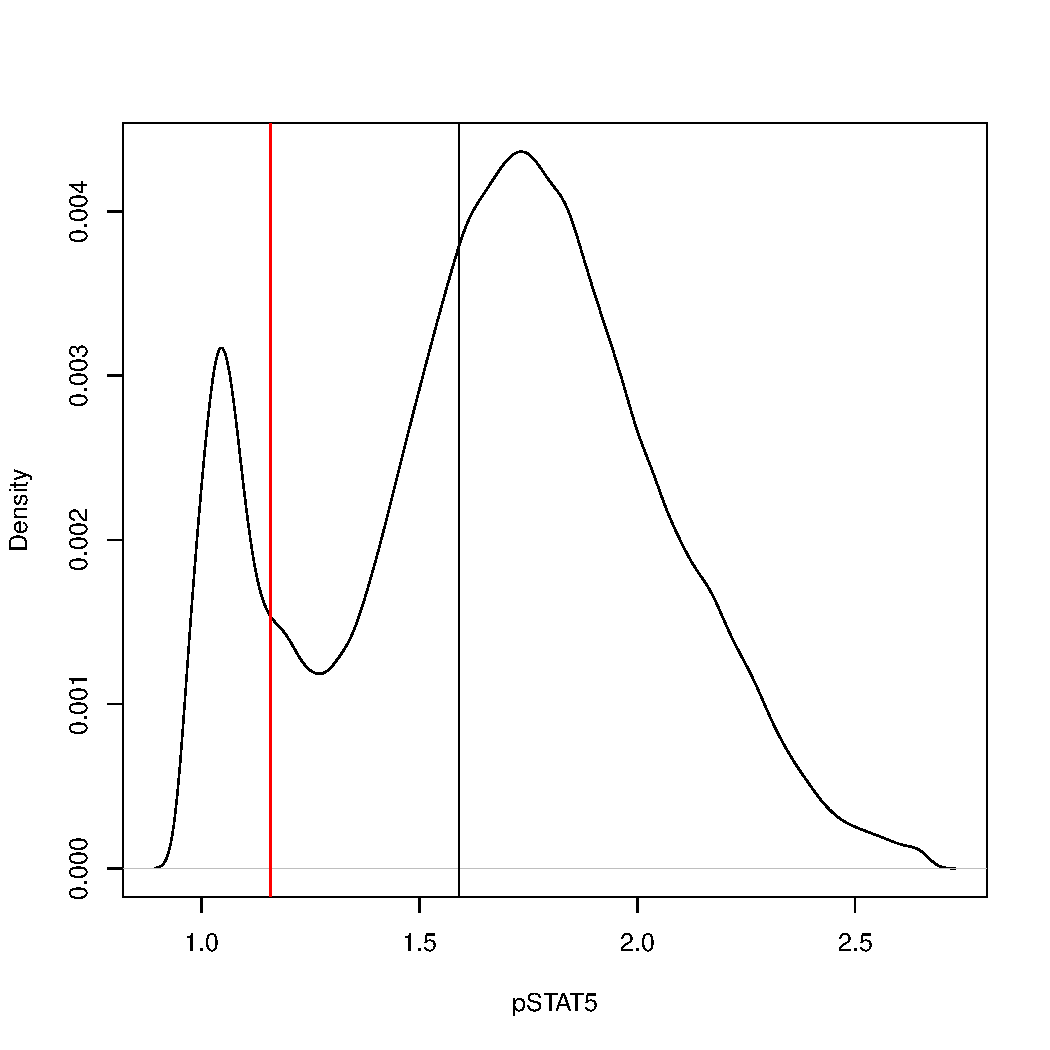
\includegraphics[scale=.5]{IL2/figures/kmeans-fail.pdf}
    %\mycaption{figure:kmeans-fail.pdf}
    %{Kmeans can fail to partition clusters when the clusters are of very uneven size (black vertical line).}
    %{
      %Fitting a mixture model allows for different cluster variance and so provides a better partitioning of the clusters.
    %}
%\end{figure}
%

